%%%% CAPÍTULO 3 - MATERIAL E MÉTODOS (PODE SER OUTRO TÍTULO DE ACORDO COM O TRABALHO REALIZADO)

\chapter{Metodologia}\label{cap:materialemetodos}

O projeto será estruturado em duas etapas principais: o desenvolvimento da
infraestrutura de \textit{hardware} e a criação do \textit{software}.
Desta forma, além da construção do protótipo físico, será desenvolvido
o programa de controle de acesso por biometria, atendendo todos
os requisitos do projeto, ou seja, desde o processamento de imagens
até o acionamento de um relé.

O fluxograma apresentado na \autoref{fig:fluxoprog} oferece uma visão
simplificada do funcionamento do \textit{software} do projeto. O sistema
de controle de acesso por biometria facial opera em dois ciclos principais:
o primeiro é dedicado à autenticação do usuário, enquanto o segundo é responsável
pelo cadastro de usuários. Além disso, há um ciclo obrigatório com um
temporizador em execução em segundo plano. Esse ciclo é ativado
automaticamente sempre que um dos ciclos principais é iniciado, com o intuito
de encerrar quaisquer atividades pendentes e prevenir possíveis \textit{loops}
dentro do sistema.

\begin{figure}[h!]
    \centering
    \caption{Fluxograma do \textit{firmware}}
    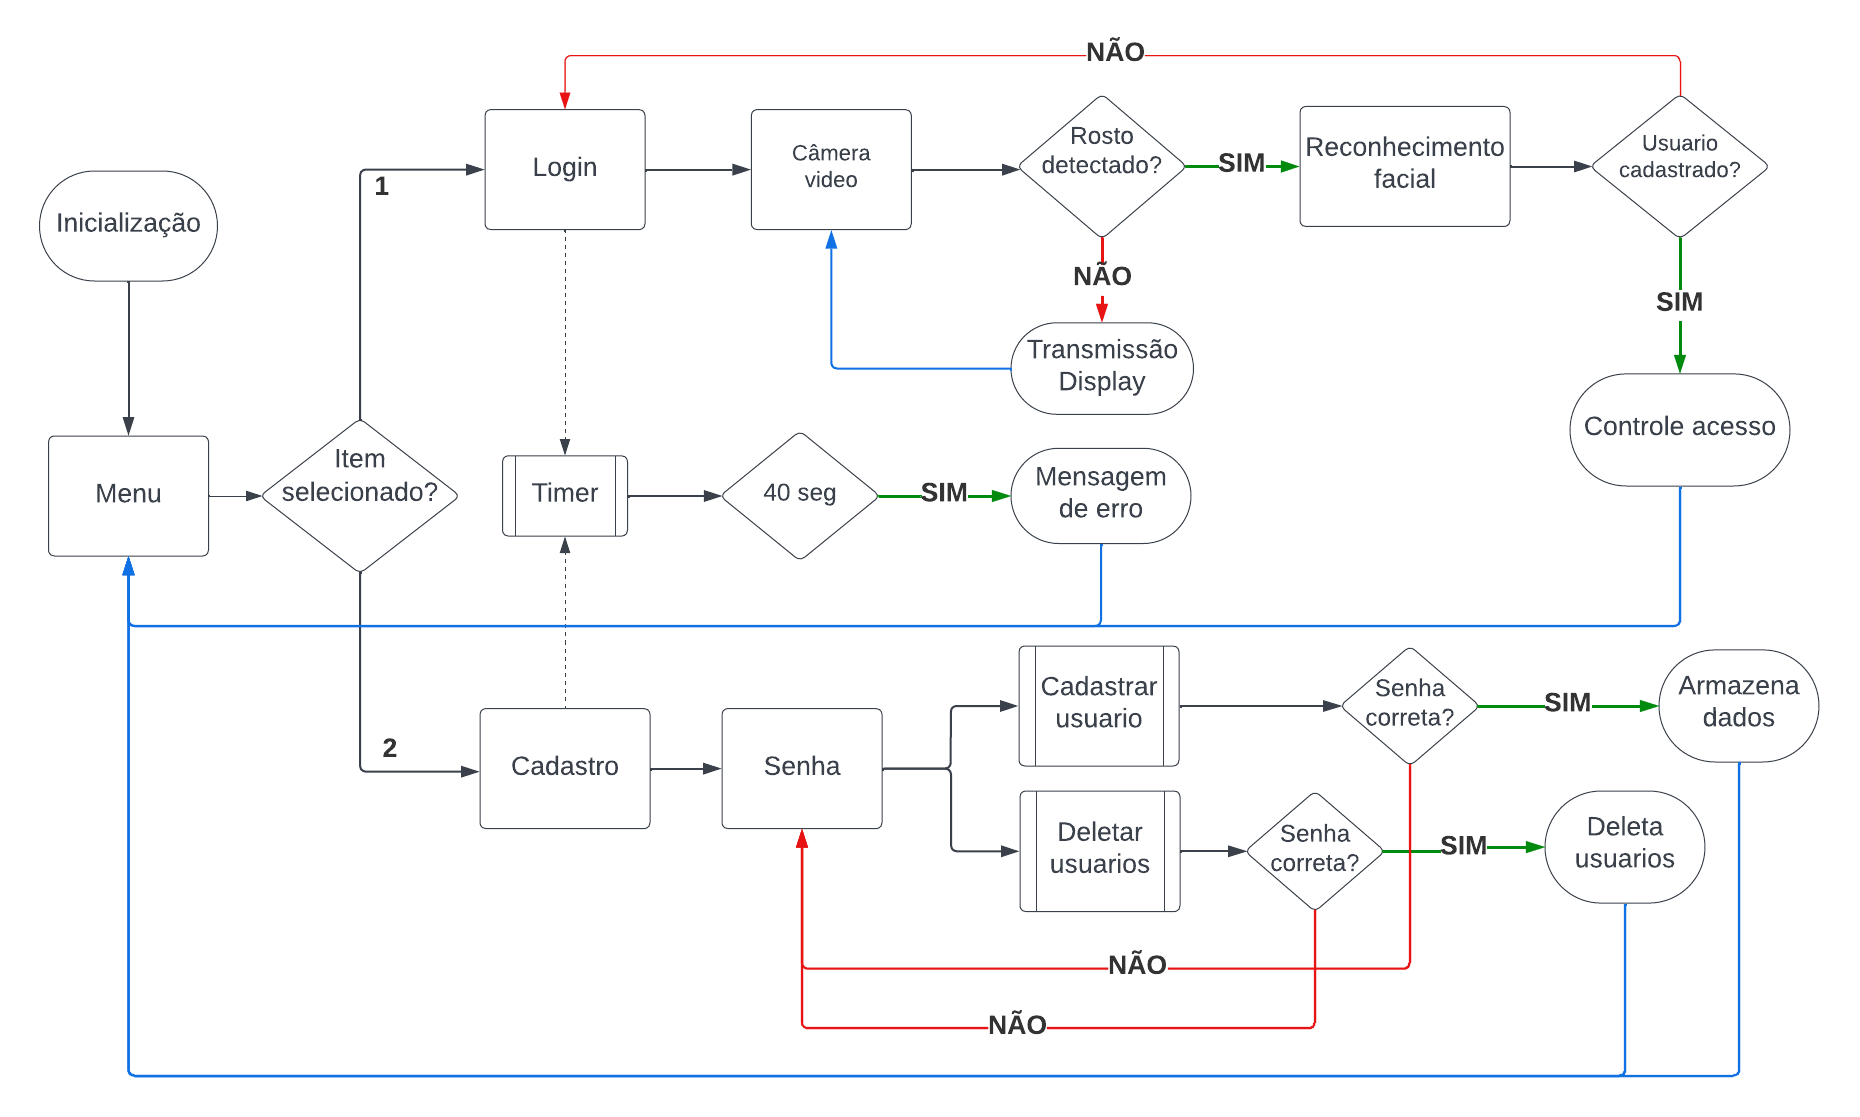
\includegraphics[scale=0.25]{figuras/fluxo_app.png}
    \fonte{}%% Fonte
    \label{fig:fluxoprog}
    \centering
\end{figure}

Para a execução desse programa, é necessário o uso de um \textit{hardware}
capaz de processá-lo. Portanto, a primeira etapa do projeto será dedicada à
construção do protótipo físico. E com o intuito de facilitar a compreensão desta
parte do projeto, foi criado o diagrama apresentado na \autoref{fig:fluxohard}.
Conforme evidenciado, o ESP32-CAM é o módulo central, encarregado do
processamento de dados e da coordenação das informações aos demais módulos.
Para melhorar a interação com os usuários, é adicionado o módulo com botões e
uma interface gráfica (display). Por fim, o módulo relé é
responsável pelo controle de acesso, podendo acionar diferentes tipos de
fechaduras elétricas.

\begin{figure}[h!]
    \centering
    \caption{Diagrama de blocos do \textit{hardware}}
    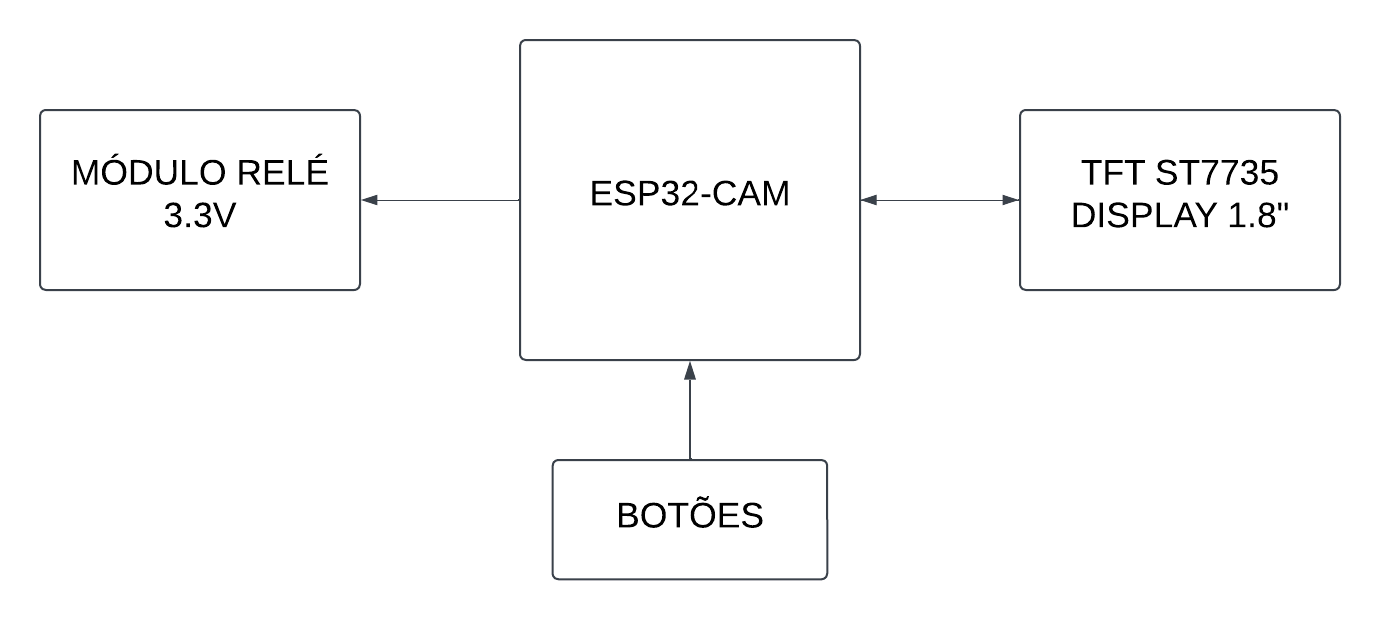
\includegraphics[scale=0.22]{figuras/diagrama_hardware.png}
    \fonte{}%% Fonte
    \label{fig:fluxohard}
    \centering
\end{figure}

Como um dos objetivos do projeto é o desenvolvimento de um protótipo de
baixo custo. A versão selecionada para essa finalidade é o ESP32-CAM,
que se destaca por integrar um \textit{chip} ESP32, uma câmera, uma
entrada para cartão SD e LED de alto brilho.

\section{Microcontrolador ESP32-CAM}\label{sec:materiais}

O ESP32-CAM (conforme ilustrado na \autoref{fig:espcam}) é um
microcontrolador de alto desempenho, desenvolvido pela empresa
\textit{Espressif Systems}® e que se destaca por sua acessibilidade.
Embora compacto, é uma escolha ideal para este projeto devido à sua
rica variedade de recursos e vantagens. Ele apresenta uma câmera
integrada à placa, um processador dual-core de 32 bits capaz de
executar tarefas em tempo real e disponibiliza 16 pinos de
Entrada/Saída (E/S).

Neste projeto, o ESP32-CAM desempenhará um papel central, sendo
responsável pelo processamento de dados, análise das informações
e controle dos demais componentes de \textit{hardware}. Isso inclui
o gerenciamento de dispositivos adicionais e a coordenação das funções
necessárias para a aplicação proposta.

\begin{figure}[h!]
    \centering
    \caption{ESP32-CAM}
    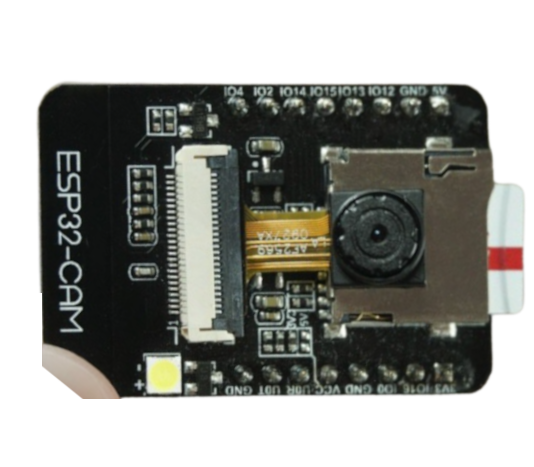
\includegraphics[scale=0.25]{figuras/esp32cam.png}
    \legend{Fonte: Adaptado de \citeonline{espcamimg}.}
    \label{fig:espcam}
    \centering
\end{figure}

\subsection{Pinos de Entrada/Saída (E/S)}\label{sec:gpio}

Os 16 pinos de Entrada/Saída (E/S) do ESP32-CAM (\autoref{fig:esp32pin})
desempenham um papel crucial na versatilidade
e funcionalidade deste microcontrolador.
Esses pinos oferecem uma interface flexível para conectar o
ESP32-CAM a uma ampla variedade de dispositivos e periféricos
externos, permitindo que ele interaja com o ambiente e execute
tarefas específicas de acordo com as necessidades do projeto.

\begin{figure}[h!]
    \centering
    \caption{GPIO disponíveis do ESP32-CAM}
    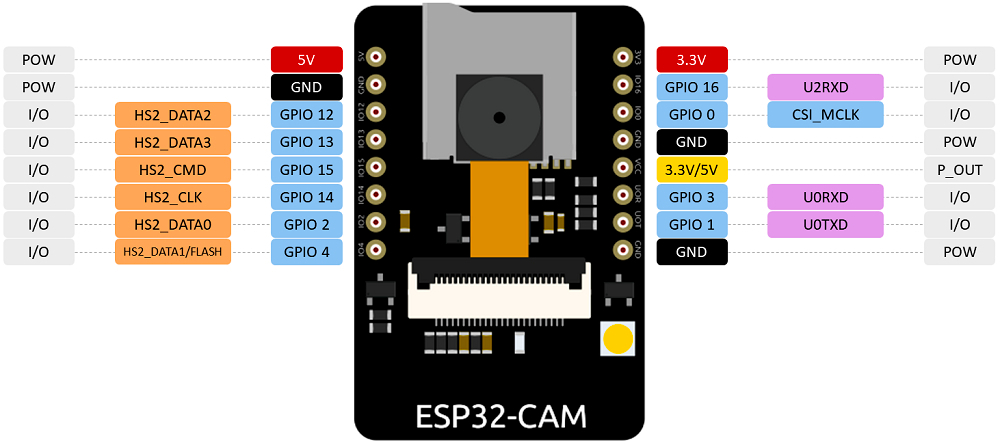
\includegraphics[scale=0.28]{figuras/esp32pin.jpg}
    \legend{Fonte: Adaptado de \citeonline{esp32pin}.}
    \label{fig:esp32pin}
    \centering
\end{figure}

Esses pinos são fundamentais para a comunicação com sensores, atuadores,
dispositivos de armazenamento, displays e muitos outros componentes
eletrônicos. Tornando o ESP32-CAM
adequado para inúmeras aplicações, desde sistemas de
segurança e monitoramento, até projetos de automação residencial..

No quadro a seguir (\autoref{quad:quadro1}), são detalhadas as funcionalidades dos 16 pinos 
de Entrada/Saída (E/S) disponíveis no ESP32-CAM. E seu entendimento, possibilita 
aos desenvolvedores a flexibilidade de personalizar e expandir suas 
aplicações de acordo com suas necessidades específicas.

\begin{tabframed}[htb]
    \caption{Portas de Entrada/Saída ESP32-CAM}
    \label{quad:quadro1}
    \begin{tabular}{|l|l|}
        \hline
        \textbf{Pinos} & \textbf{Descrição}                                                                          \\ \hline
        5V             & Pino de entrada para alimentação do circuito do ESP32.                                      \\ \hline
        3GND           & 3 pinos de aterramento, usado para referência de potencial zero                             \\ \hline
        GPIO12         & Pino de propósito geral.                                                                    \\ \hline
        GPIO13         & Pino de propósito geral.                                                                    \\ \hline
        GPIO15         & Pino de propósito geral.                                                                    \\ \hline
        GPIO14         & Pino de propósito geral.                                                                    \\ \hline
        GPIO2          & Pino de propósito geral.                                                                    \\ \hline
        GPIO4          & Pino de propósito geral e pode ser utilizado para acionar o Flash do ESP32.                 \\ \hline
        3.3V           & Pino de fornecimento de energia de 3,3V.                                                    \\ \hline
        GPIO16         & Este pino sempre fica em nível lógico alto e é utilizado para alimentar o circuto de PSRAM. \\ \hline
        GPIO0          & Pino de propósito geral, entretanto este pino é responsável pelo clock da cÂmera.           \\ \hline
        3.3V/5V        & Pode fornecer energia de 3,3V ou 5V para outros dispositivos.                               \\ \hline
        GPIO3          & Pino de entrada de dados UART (RX) para comunicação serial.                                 \\ \hline
        GPIO1          & Pino de saída de dados UART (TX) para comunicação serial.                                   \\ \hline
    \end{tabular}
    \fonte{}%% Fonte
\end{tabframed}

\section{Interface gráfica}\label{sec:interface}

O Display LCD TFT de 1.8 polegadas, com resolução de 128x160 pixels
e \textit{driver} ST7735 (\autoref{fig:tft7735}) é um componente popular 
utilizado em uma variedade de aplicações eletrônicas, devido à sua 
capacidade de fornecer uma interface visual clara e interativa. 
Esse tipo de display é frequentemente empregado em projetos que requerem 
a exibição de informações, gráficos e interação direta com o usuário.

Neste contexto, o uso deste display no projeto tem o propósito de aprimorar 
a experiência do usuário, fornecendo uma representação visual clara da 
aplicação. Além disso, sua biblioteca de fácil utilização simplifica o 
processo de desenvolvimento do projeto, tornando-o mais acessível e eficaz.

\begin{figure}[h!]
    \centering
    \caption{Display LCD TFT 1.8"}
    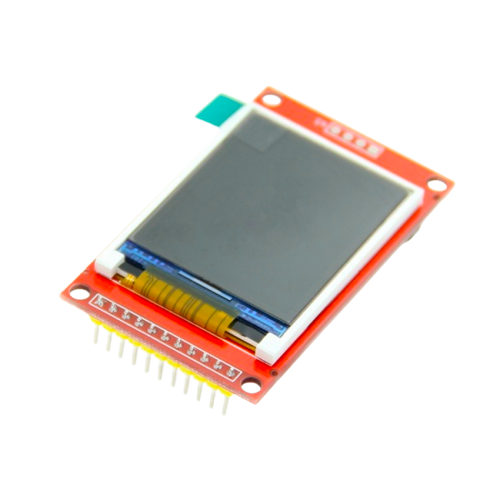
\includegraphics[scale=0.5]{figuras/tftst7735.png}
    \legend{Fonte: Adaptado de \citeonline{tft7735img}.}
    \label{fig:tft7735}
    \centering
\end{figure}

\section{Módulo de acionamento}\label{sec:acionamento}

Um módulo relé, como por exemplo, o da \autoref{fig:rele}, é um componente 
eletrônico amplamente utilizado em projetos que envolvem controle 
e automação de dispositivos elétricos. Ele desempenha 
um papel essencial ao permitir o controle de circuitos 
de alta potência por meio de sinais de baixa potência.

\begin{figure}[h!]
    \centering
    \caption{Módulo Relé}
    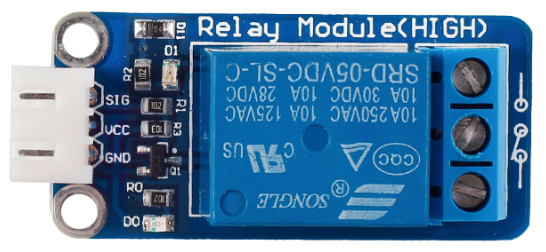
\includegraphics[scale=1]{figuras/rele.png}
    \fonte{\citeonline{releimg}}%% Fonte \legend{Fonte: Adaptado de \citeonline{releimg}.}
    \label{fig:rele}
    \centering
\end{figure}

Quando se trata de fechaduras eletrônicas, como o da \autoref{fig:fecho}, 
os módulos relé desempenham um papel crucial, facilitando o funcionamento e 
a segurança do sistema de controle de acesso. Geralmente, essas fechaduras 
incluem um mecanismo de trinco que pode ser controlado eletronicamente. 
O módulo relé é utilizado para controlar a ativação e desativação 
desse mecanismo. Quando um usuário autorizado fornece uma credencial 
válida (como uma senha, cartão RFID ou impressão digital), o sistema 
eletrônico de controle gera um sinal de baixa potência para acionar 
o módulo relé. O relé fecha seu contato, permitindo a passagem de 
energia para o mecanismo de destravamento da fechadura, liberando 
assim o acesso.

\begin{figure}[h!]
    \centering
    \caption{Fecho Elétrico}
    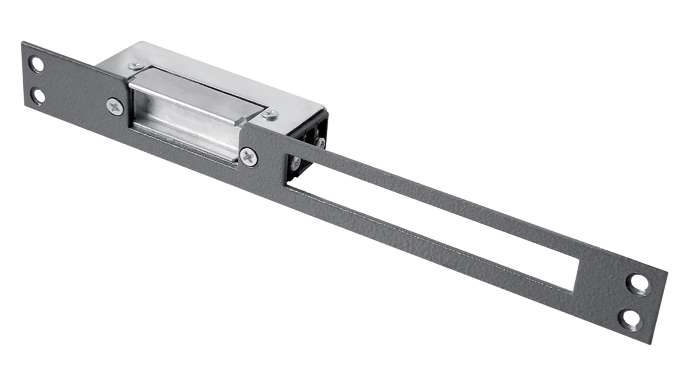
\includegraphics[scale=0.25]{figuras/fechoagl.png}
    \fonte{\citeonline{fechaduraimg}}%%\legend{Fonte: Adaptado de \citeonline{fechaduraimg}.}
    \label{fig:fecho}
    \centering
\end{figure}

\section{Desenvolvimento do software}\label{sec:software}

Para o desenvolvimento do software, foi essencial escolher uma plataforma 
de desenvolvimento capaz de programar e gravar códigos nos microcontroladores 
ESP32. Duas opções amplamente conhecidas são o Arduino IDE e o PlatformIO. 
Além disso, o desenvolvimento exigiu um estudo aprofundado das 
bibliotecas disponíveis para atender aos requisitos do projeto, 
tais como o reconhecimento facial, transmissão em tempo real de 
imagens em um display LCD, implementação de um timer e a manipulação 
dos dados de entrada e saída.

\subsection{PlatformIO}\label{sec:platformio}

A plataforma escolhida para esse projeto foi o PlatformIO, 
que é uma ferramenta indispensável para quem trabalha com dispositivos 
microcontrolados, como o ESP32. Projetado para simplificar o processo 
de desenvolvimento e programação de microcontroladores, o PlatformIO 
oferece uma ampla gama de recursos e uma abordagem unificada que 
facilita o trabalho com diferentes plataformas de hardware e 
ambientes de desenvolvimento.

Quando se trata do ESP32, o PlatformIO desempenha 
um papel crucial, permitindo que desenvolvedores e entusiastas de 
eletrônica programem e depurem suas aplicações de maneira eficiente.
O PlatformIO é projetado para funcionar com diversos editores de 
código populares, como Visual Studio Code (VSCode), Atom e CLion. 
Isso permite que os desenvolvedores escolham a IDE que melhor 
se adapte às suas preferências.

Por fim, dois outros pontos fortes do PlatformIO é que ele 
possui um gerenciador de bibliotecas embutido que facilita a 
pesquisa, instalação e atualização de bibliotecas de código-fonte 
aberto. Isso é particularmente útil para reutilizar código 
existente e acelerar o desenvolvimento. Como também sua 
simplificação no processo de compilação e carregamento de 
código para o hardware de destino. 

\subsection{Biblioteca ESP-DL}\label{sec:formatacaoTexto}

Para identificação de rostos e reconhecimento facial, foram utilizados 
os recursos disponíveis da biblioteca ESP-DL.

O ESP-DL é uma biblioteca de alto desempenho dedicada ao ESP32, ESP32-S2,
ESP32-S3 e ESP32-C3, projetada para recursos de aprendizagem profunda.

O \citeonline{espdl} disponibiliza APIs para tarefas como inferência 
de redes neurais (NN), processamento de imagens, operações matemáticas 
e inclui alguns modelos de aprendizado profundo. Com essa biblioteca, 
os desenvolvedores podem aproveitar os SoCs (System-on-Chip) da 
\textit{Espressif} de maneira simples e ágil para a implementação 
de uma ampla variedade de aplicações.

Dentre os recursos disponíveis do ESP-DL, se encontra o 
ESP-Face, componente que fornece funções de detecção e 
reconhecimento facial e também operações de rede neural. 
O método \textit{face detect} utiliza o modelo MTMN (\textit{Multi-Task 
Memory Network}) para a detecção de rostos humanos. 
Esse modelo, especialmente projetado para dispositivos 
embarcados, apresenta uma operação eficiente que se 
baseia na arquitetura móvel MobileNetV2 e utiliza 
redes convolucionais em cascata multitarefa.

O MobileNetV2 faz parte de uma nova geração de redes 
neurais convolucionais profundas voltadas para a 
visão computacional. Essa arquitetura permite a 
implementação em tempo real de aplicativos de 
classificação, detecção e alinhamento de objetos 
em dispositivos móveis pessoais, destacando-se por 
sua capacidade de processamento leve.

O MTMN se beneficia de redes neurais pré-treinadas, 
que foram desenvolvidas com base em um vasto banco de 
dados contendo mais de um milhão de imagens do ImageNet. 
Essas redes aprenderam representações de recursos de 
mais de 1.000 categorias de objetos, fornecendo uma 
base sólida para a detecção de rostos.

Uma característica distintiva do MTMN é sua estrutura 
multitarefa de aprendizagem em cascata. Essa abordagem 
permite que o modelo resolva desafios encontrados em 
ambientes diversos, como variações de iluminação, 
oclusões e poses variadas. O MTMN é composto por três 
estágios de redes convolucionais profundas que preveem a 
localização de faces e pontos de referência, proporcionando 
uma detecção precisa que varia de informações gerais a 
detalhes específicos.

No contexto do reconhecimento facial, uma vez que um rosto 
humano tenha sido detectado por meio do procedimento 
mencionado anteriormente, é possível realizar uma verificação 
comparando-o com os rostos previamente cadastrados. 
A entrada para esse processo é a imagem original juntamente 
com os resultados obtidos na etapa de detecção facial.

O método de reconhecimento facial, denominado "recognize face" 
faz uso do modelo FRMN (\textit{Face Recognition Memory Network}), que 
também se baseia na arquitetura móvel MobileNetV2 e emprega o 
algoritmo ArcFace. Para otimizar a complexidade computacional, 
as imagens foram treinadas em dimensões reduzidas (56x56).

Esse procedimento, além de oferecer um processo de reconhecimento 
facial eficiente, permite a comparação precisa entre o rosto 
identificado e as informações previamente cadastradas, 
contribuindo para uma solução de alta qualidade em sistemas 
de identificação e autenticação.

\subsection{Fluxo de telas}\label{sec:telas}

Os recursos gráficos fornecidos pelo display LCD desempenham um papel 
fundamental na usabilidade da aplicação. Nesse contexto, a elaboração 
do fluxo de telas se torna essencial para proporcionar aos usuários 
uma experiência eficiente. Todos os fluxos foram planejados e 
projetados com o objetivo de guiar o usuário por meio 
de diferentes interações e funcionalidades.

O primeiro conjunto de telas (\autoref{fig:fluxoinicial}), referente à 
inicialização dos recursos utilizados no programa do protótipo, 
abrange o momento em que a câmera, os sensores e o SPIFFS 
(Sistema de Arquivos Flash de Interface Serial Periférica) 
são ativados. Além disso, a lista de usuários cadastrados é 
inicializada antes de exibir a tela de menu." 

\begin{figure}[h!]
    \centering
    \caption{Telas de inicialização}
    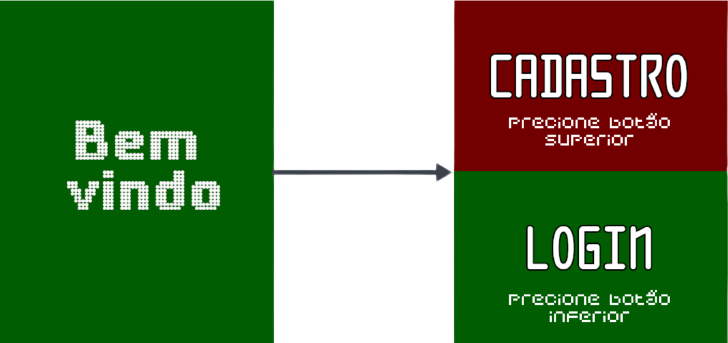
\includegraphics[scale=0.3]{figuras/fluxo_inicial.png}
    \fonte{}%% Fonte
    \label{fig:fluxoinicial}
    \centering
\end{figure}

Ao chegar ao menu e selecionar a opção de login, o usuário inicia o 
fluxo de telas de login. Inicialmente, é exibida uma mensagem de 
orientação para enquadrar o rosto dentro do campo de visão da câmera. 
Se o usuário estiver cadastrado, uma mensagem de sucesso é exibida, 
e em seguida, o módulo do relé é acionado. Caso contrário, o timer 
é executado em segundo plano, e quando o tempo se esgota, uma mensagem 
de erro é exibida, como representado na \autoref{fig:fluxologin}.

\begin{figure}[h!]
    \centering
    \caption{Fluxo de telas do login}
    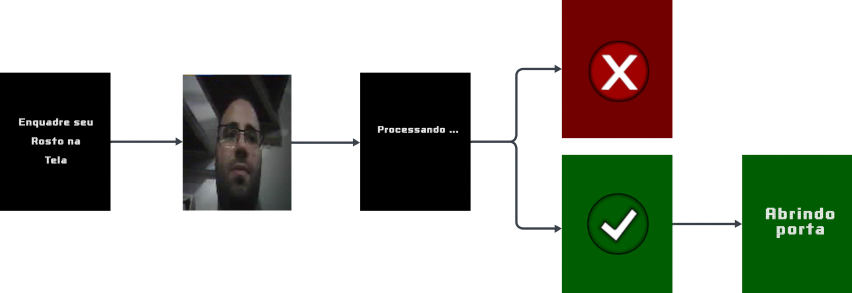
\includegraphics[scale=2.2]{figuras/fluxo_login.png}
    \fonte{}%% Fonte
    \label{fig:fluxologin}
    \centering
\end{figure}

No entanto, se o usuário escolher a opção de cadastro no menu, 
ele deverá seguir o fluxo descrito na \autoref{fig:fluxocadastro}. 
Na primeira etapa, o usuário é solicitado a digitar a senha. 
Se a senha estiver correta, uma mensagem de "senha correta" é 
exibida, e o processo de identificação e reconhecimento facial 
é iniciado. Se tudo ocorrer conforme o esperado, os dados são 
armazenados na memória RAM ou na memória flash. Caso contrário, 
o usuário visualizará uma mensagem de erro.

\begin{figure}[h!]
    \centering
    \caption{Fluxo de telas do cadastro}
    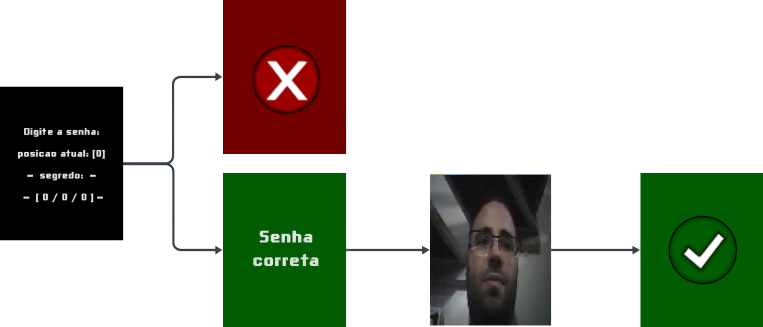
\includegraphics[scale=2.5]{figuras/fluxo_cadastro.png}
    \fonte{}%% Fonte
    \label{fig:fluxocadastro}
    \centering
\end{figure}


Por fim, o ultimo fluxo principal é o processo de exclusão 
de usuários (\autoref{fig:fluxosenha}), que se assemelha 
muito ao fluxo de cadastro. Como observado, em ambos 
os casos, a primeira tela solicita a inserção 
da senha, e o usuário tem aproximadamente 40 segundos 
para descobrir ou digitar a senha correta. Durante esse processo, 
podem ser exibidas mensagens de erro ou sucesso. Se tudo ocorrer 
conforme o esperado, a mensagem "usuários deletados" é exibida.

\begin{figure}[h!]
    \centering
    \caption{Telas deletar usuario}
    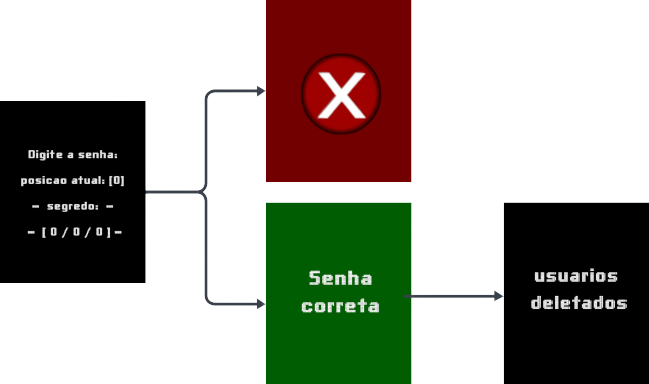
\includegraphics[scale=2.5]{figuras/fluxo_deletar_usuario.png}
    \fonte{}%% Fonte
    \label{fig:fluxosenha}
    \centering
\end{figure}

\section{Desenvolvimento do protótipo}\label{sec:prototipo}

Para o desenvolvimento do protótipo foi necessário utilizar uma caixa

Devido ao tamanho reduzido da caixa, foi necessário realizar um projeto minucioso de
criação 3D seguindo as medidas exatas para que fosse possível alocar todos os conectores, botões
e o circuito em si. Dessa forma, com a caixa modelada 3D foi possível testar as melhores posições
para todos os elementos e também ter a medida e modelo exato para a placa de circuito impresso.

O passo seguinte foi a criação do diagrama elétrico final do protótipo, mostrado na Figura
36, feito com base no circuito testado e montado na protoboard. Optou-se pela inclusão de
conectores do tipo KK que possuem travas para evitar desconexões


\begin{figure}[h!]
    \centering
    \caption{Diagrama elétrico do protótipo}
    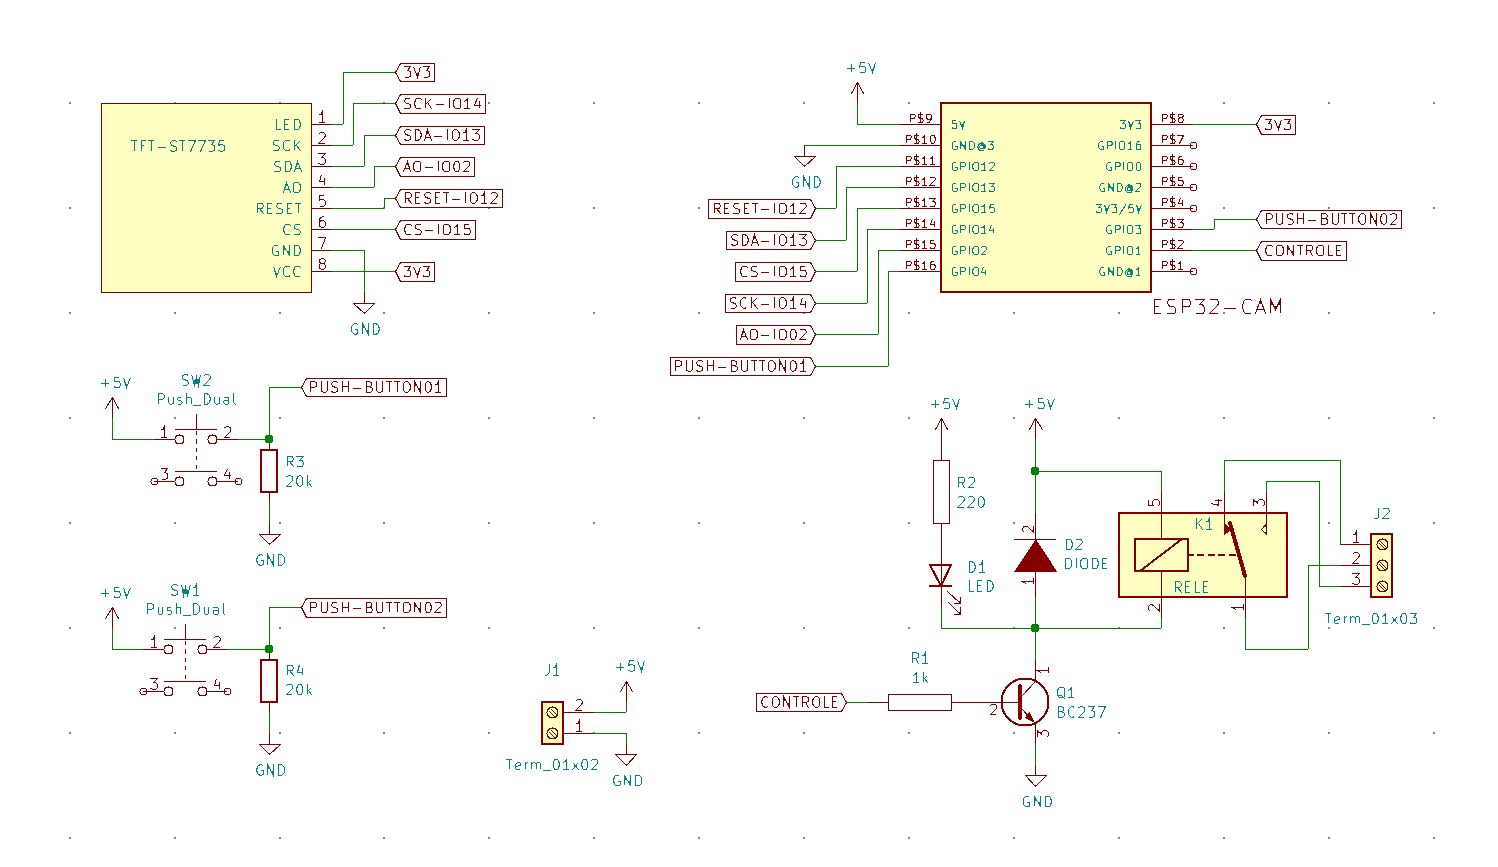
\includegraphics[scale=0.3]{figuras/circuito_completo.png}
    \fonte{}%% Fonte
    \label{fig:circuito}
    \centering
\end{figure}

Com base no esquema e no dimensionamento possível, a placa em dupla face foi criada,
como mostra a Figura 37, onde os recortes foram necessários para que fosse possível encaixar os
conectores da caixa. Além disso, a parte de botões da placa foi feita de forma destacável, uma
vez que no projeto ela se encontra acima da placa principal, fixada na caixa.

\begin{figure}[h!]
    \centering
    \caption{Diagrama elétrico do Display TFT}
    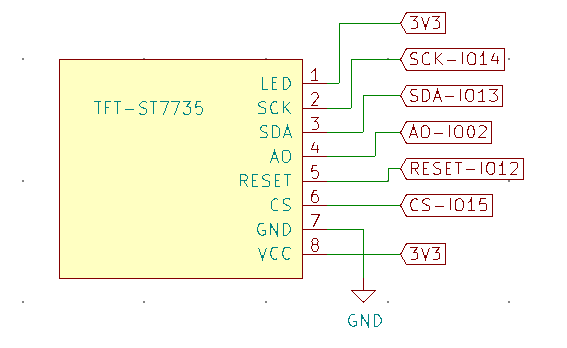
\includegraphics[scale=0.4]{figuras/modulo_tft.png}
    \fonte{}%% Fonte
    \label{fig:diagramatft}
    \centering
\end{figure}

\begin{figure}[h!]
    \centering
    \caption{Diagrama elétrico do ESP32-CAM}
    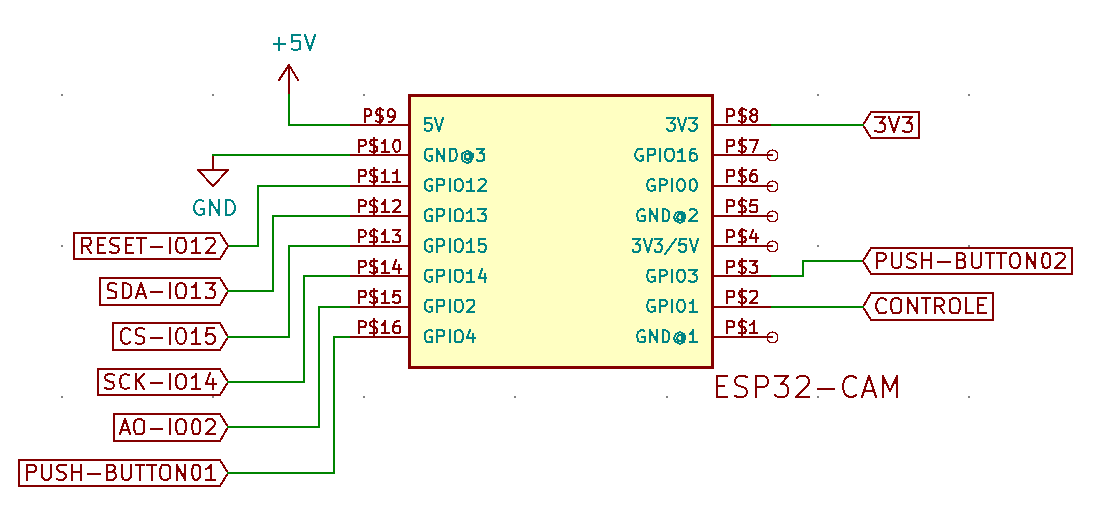
\includegraphics[scale=0.35]{figuras/modulo_esp.png}
    \fonte{}%% Fonte
    \label{fig:diagramaesp}
    \centering
\end{figure}

\begin{figure}[h!]
    \centering
    \caption{Diagrama elétrico dos botões}
    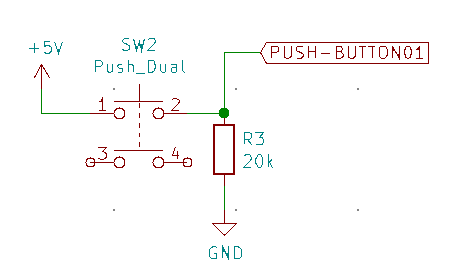
\includegraphics[scale=0.4]{figuras/modulo-push-button.png}
    \fonte{}%% Fonte
    \label{fig:diagramabotoes}
    \centering
\end{figure}

\begin{figure}[h!]
    \centering
    \caption{Diagrama elétrico acionamento relé}
    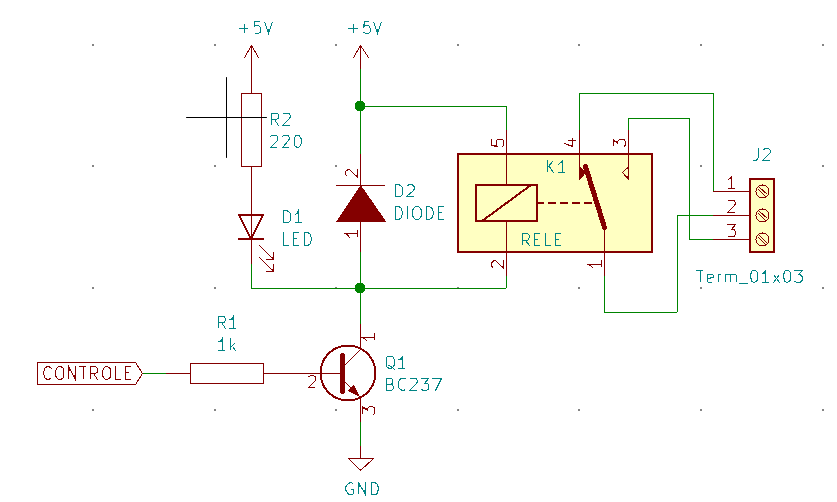
\includegraphics[scale=0.4]{figuras/modulo_rele_esquema.png}
    \fonte{}%% Fonte
    \label{fig:diagramarele}
    \centering
\end{figure}


\begin{figure}[h!]
    \centering
    \caption{Projeto da placa de circuito impresso do protótipo}
    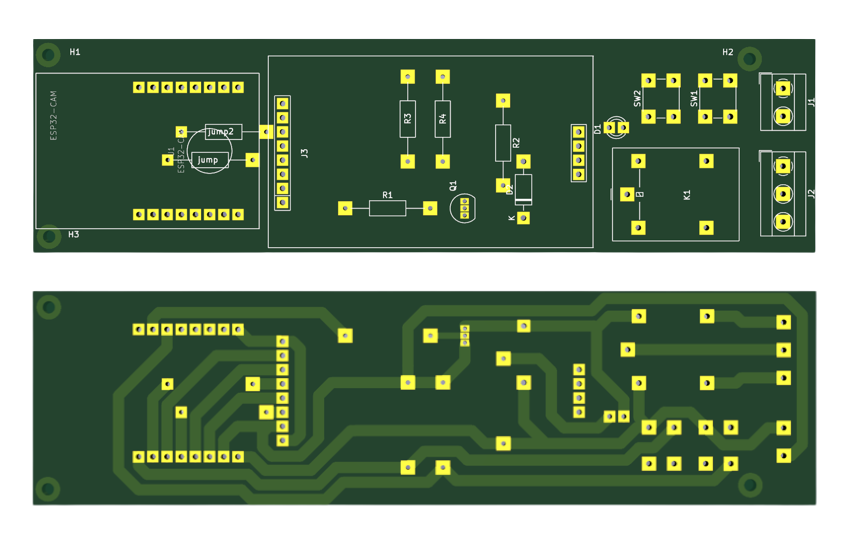
\includegraphics[scale=0.35]{figuras/placa_pcb.png}
    \fonte{}%% Fonte
    \label{fig:placapcb}
    \centering
\end{figure}

\begin{figure}[h!]
    \centering
    \caption{Placa manufaturada}
    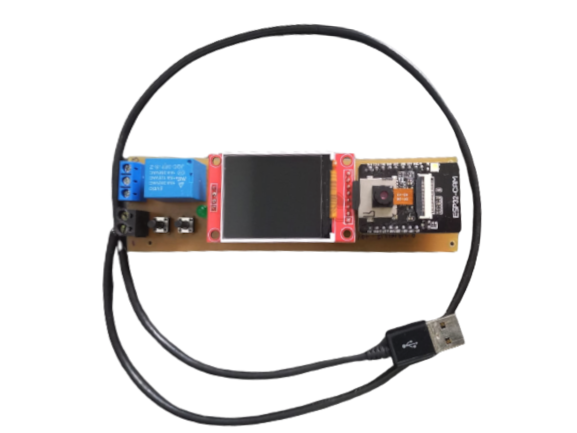
\includegraphics[scale=0.45]{figuras/placa_montada.png}
    \fonte{}%% Fonte
    \label{fig:placamanufaturada}
    \centering
\end{figure}

\begin{figure}[h!]
    \centering
    \caption{Placa montada}
    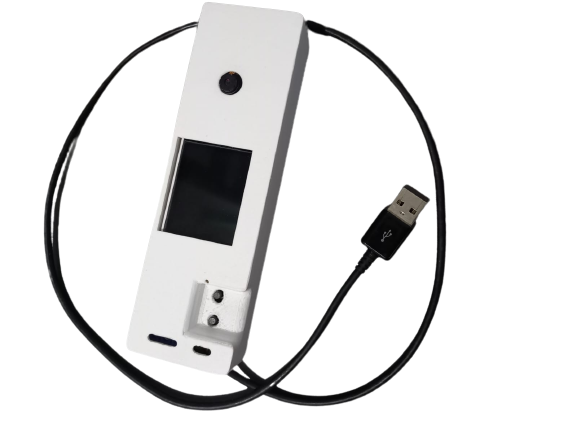
\includegraphics[scale=0.3]{placa_case.png}
    \fonte{}%% Fonte
    \label{fig:placamontada}
    \centering
\end{figure}